% Options for packages loaded elsewhere
\PassOptionsToPackage{unicode}{hyperref}
\PassOptionsToPackage{hyphens}{url}
%
\documentclass[
]{article}
\usepackage{lmodern}
\usepackage{amssymb,amsmath}
\usepackage{ifxetex,ifluatex}
\ifnum 0\ifxetex 1\fi\ifluatex 1\fi=0 % if pdftex
  \usepackage[T1]{fontenc}
  \usepackage[utf8]{inputenc}
  \usepackage{textcomp} % provide euro and other symbols
\else % if luatex or xetex
  \usepackage{unicode-math}
  \defaultfontfeatures{Scale=MatchLowercase}
  \defaultfontfeatures[\rmfamily]{Ligatures=TeX,Scale=1}
\fi
% Use upquote if available, for straight quotes in verbatim environments
\IfFileExists{upquote.sty}{\usepackage{upquote}}{}
\IfFileExists{microtype.sty}{% use microtype if available
  \usepackage[]{microtype}
  \UseMicrotypeSet[protrusion]{basicmath} % disable protrusion for tt fonts
}{}
\makeatletter
\@ifundefined{KOMAClassName}{% if non-KOMA class
  \IfFileExists{parskip.sty}{%
    \usepackage{parskip}
  }{% else
    \setlength{\parindent}{0pt}
    \setlength{\parskip}{6pt plus 2pt minus 1pt}}
}{% if KOMA class
  \KOMAoptions{parskip=half}}
\makeatother
\usepackage{xcolor}
\IfFileExists{xurl.sty}{\usepackage{xurl}}{} % add URL line breaks if available
\IfFileExists{bookmark.sty}{\usepackage{bookmark}}{\usepackage{hyperref}}
\hypersetup{
  pdftitle={Results of PangoVis},
  pdfauthor={Devan Becker},
  hidelinks,
  pdfcreator={LaTeX via pandoc}}
\urlstyle{same} % disable monospaced font for URLs
\usepackage[margin=1in]{geometry}
\usepackage{color}
\usepackage{fancyvrb}
\newcommand{\VerbBar}{|}
\newcommand{\VERB}{\Verb[commandchars=\\\{\}]}
\DefineVerbatimEnvironment{Highlighting}{Verbatim}{commandchars=\\\{\}}
% Add ',fontsize=\small' for more characters per line
\usepackage{framed}
\definecolor{shadecolor}{RGB}{248,248,248}
\newenvironment{Shaded}{\begin{snugshade}}{\end{snugshade}}
\newcommand{\AlertTok}[1]{\textcolor[rgb]{0.94,0.16,0.16}{#1}}
\newcommand{\AnnotationTok}[1]{\textcolor[rgb]{0.56,0.35,0.01}{\textbf{\textit{#1}}}}
\newcommand{\AttributeTok}[1]{\textcolor[rgb]{0.77,0.63,0.00}{#1}}
\newcommand{\BaseNTok}[1]{\textcolor[rgb]{0.00,0.00,0.81}{#1}}
\newcommand{\BuiltInTok}[1]{#1}
\newcommand{\CharTok}[1]{\textcolor[rgb]{0.31,0.60,0.02}{#1}}
\newcommand{\CommentTok}[1]{\textcolor[rgb]{0.56,0.35,0.01}{\textit{#1}}}
\newcommand{\CommentVarTok}[1]{\textcolor[rgb]{0.56,0.35,0.01}{\textbf{\textit{#1}}}}
\newcommand{\ConstantTok}[1]{\textcolor[rgb]{0.00,0.00,0.00}{#1}}
\newcommand{\ControlFlowTok}[1]{\textcolor[rgb]{0.13,0.29,0.53}{\textbf{#1}}}
\newcommand{\DataTypeTok}[1]{\textcolor[rgb]{0.13,0.29,0.53}{#1}}
\newcommand{\DecValTok}[1]{\textcolor[rgb]{0.00,0.00,0.81}{#1}}
\newcommand{\DocumentationTok}[1]{\textcolor[rgb]{0.56,0.35,0.01}{\textbf{\textit{#1}}}}
\newcommand{\ErrorTok}[1]{\textcolor[rgb]{0.64,0.00,0.00}{\textbf{#1}}}
\newcommand{\ExtensionTok}[1]{#1}
\newcommand{\FloatTok}[1]{\textcolor[rgb]{0.00,0.00,0.81}{#1}}
\newcommand{\FunctionTok}[1]{\textcolor[rgb]{0.00,0.00,0.00}{#1}}
\newcommand{\ImportTok}[1]{#1}
\newcommand{\InformationTok}[1]{\textcolor[rgb]{0.56,0.35,0.01}{\textbf{\textit{#1}}}}
\newcommand{\KeywordTok}[1]{\textcolor[rgb]{0.13,0.29,0.53}{\textbf{#1}}}
\newcommand{\NormalTok}[1]{#1}
\newcommand{\OperatorTok}[1]{\textcolor[rgb]{0.81,0.36,0.00}{\textbf{#1}}}
\newcommand{\OtherTok}[1]{\textcolor[rgb]{0.56,0.35,0.01}{#1}}
\newcommand{\PreprocessorTok}[1]{\textcolor[rgb]{0.56,0.35,0.01}{\textit{#1}}}
\newcommand{\RegionMarkerTok}[1]{#1}
\newcommand{\SpecialCharTok}[1]{\textcolor[rgb]{0.00,0.00,0.00}{#1}}
\newcommand{\SpecialStringTok}[1]{\textcolor[rgb]{0.31,0.60,0.02}{#1}}
\newcommand{\StringTok}[1]{\textcolor[rgb]{0.31,0.60,0.02}{#1}}
\newcommand{\VariableTok}[1]{\textcolor[rgb]{0.00,0.00,0.00}{#1}}
\newcommand{\VerbatimStringTok}[1]{\textcolor[rgb]{0.31,0.60,0.02}{#1}}
\newcommand{\WarningTok}[1]{\textcolor[rgb]{0.56,0.35,0.01}{\textbf{\textit{#1}}}}
\usepackage{graphicx}
\makeatletter
\def\maxwidth{\ifdim\Gin@nat@width>\linewidth\linewidth\else\Gin@nat@width\fi}
\def\maxheight{\ifdim\Gin@nat@height>\textheight\textheight\else\Gin@nat@height\fi}
\makeatother
% Scale images if necessary, so that they will not overflow the page
% margins by default, and it is still possible to overwrite the defaults
% using explicit options in \includegraphics[width, height, ...]{}
\setkeys{Gin}{width=\maxwidth,height=\maxheight,keepaspectratio}
% Set default figure placement to htbp
\makeatletter
\def\fps@figure{htbp}
\makeatother
\setlength{\emergencystretch}{3em} % prevent overfull lines
\providecommand{\tightlist}{%
  \setlength{\itemsep}{0pt}\setlength{\parskip}{0pt}}
\setcounter{secnumdepth}{-\maxdimen} % remove section numbering
\usepackage[]{natbib}
\bibliographystyle{plainnat}

\title{Results of PangoVis}
\author{Devan Becker}
\date{2021-03-31}

\begin{document}
\maketitle

\hypertarget{load-packages-and-data}{%
\section{Load Packages and Data}\label{load-packages-and-data}}

\begin{Shaded}
\begin{Highlighting}[]
\CommentTok{\# Packages that Art hates}
\KeywordTok{library}\NormalTok{(dplyr)}
\end{Highlighting}
\end{Shaded}

\begin{verbatim}
## 
## Attaching package: 'dplyr'
\end{verbatim}

\begin{verbatim}
## The following objects are masked from 'package:stats':
## 
##     filter, lag
\end{verbatim}

\begin{verbatim}
## The following objects are masked from 'package:base':
## 
##     intersect, setdiff, setequal, union
\end{verbatim}

\begin{Shaded}
\begin{Highlighting}[]
\KeywordTok{library}\NormalTok{(tidyr)}
\KeywordTok{library}\NormalTok{(ggplot2)}
\KeywordTok{library}\NormalTok{(stringr)}
\KeywordTok{library}\NormalTok{(here)}
\end{Highlighting}
\end{Shaded}

\begin{verbatim}
## here() starts at /home/devan/OneDriveUWO/0postdoc/sup
\end{verbatim}

\begin{Shaded}
\begin{Highlighting}[]
\NormalTok{dirich \textless{}{-}}\StringTok{ }\NormalTok{params}\OperatorTok{$}\NormalTok{dirich}

\CommentTok{\# Read in CSV files}
\NormalTok{csvs \textless{}{-}}\StringTok{ }\KeywordTok{list.files}\NormalTok{(}\StringTok{"../data/pangolineages"}\NormalTok{, }
    \DataTypeTok{pattern =} \KeywordTok{ifelse}\NormalTok{(dirich, }\StringTok{"*\_d.csv"}\NormalTok{, }\StringTok{"*.csv"}\NormalTok{), }
    \DataTypeTok{full.names =} \OtherTok{TRUE}\NormalTok{)}

\CommentTok{\# Remove any copies}
\NormalTok{csvs \textless{}{-}}\StringTok{ }\NormalTok{csvs[}\OperatorTok{!}\KeywordTok{grepl}\NormalTok{(}\StringTok{"{-}1"}\NormalTok{, csvs)]}
\CommentTok{\# Proper names}
\CommentTok{\#csvs \textless{}{-} paste0("../data/pangolineages/", csvs)}

\CommentTok{\# Bring them into one data frame}
\NormalTok{lins \textless{}{-}}\StringTok{ }\KeywordTok{bind\_rows}\NormalTok{(}\KeywordTok{lapply}\NormalTok{(csvs, read.csv))}

\CommentTok{\# Taxon is encoded as \_ACCSESSIONNUMBER.ID, split into ACCESSIONNUMBER and ID}
\NormalTok{lins \textless{}{-}}\StringTok{ }\NormalTok{lins }\OperatorTok{\%\textgreater{}\%}\StringTok{ }
\StringTok{    }\KeywordTok{separate}\NormalTok{(}\DataTypeTok{col =} \StringTok{"taxon"}\NormalTok{, }\DataTypeTok{sep =} \StringTok{"}\CharTok{\textbackslash{}\textbackslash{}}\StringTok{."}\NormalTok{, }
        \DataTypeTok{into =} \KeywordTok{c}\NormalTok{(}\StringTok{"taxon"}\NormalTok{, }\StringTok{"sample"}\NormalTok{)) }\OperatorTok{\%\textgreater{}\%}\StringTok{ }
\StringTok{    }\KeywordTok{mutate}\NormalTok{(}\DataTypeTok{taxon =} \KeywordTok{str\_replace}\NormalTok{(taxon, }\StringTok{"}\CharTok{\textbackslash{}\textbackslash{}}\StringTok{\_"}\NormalTok{, }\StringTok{""}\NormalTok{))}

\CommentTok{\#\#\#\# Visualize the uncertainty in the base calls {-}{-}{-}{-}}
\NormalTok{taxons \textless{}{-}}\StringTok{ }\KeywordTok{unique}\NormalTok{(lins}\OperatorTok{$}\NormalTok{taxon)}
\KeywordTok{length}\NormalTok{(taxons)}
\end{Highlighting}
\end{Shaded}

\begin{verbatim}
## [1] 36
\end{verbatim}

\hypertarget{abstract-info}{%
\section{Abstract Info}\label{abstract-info}}

\begin{Shaded}
\begin{Highlighting}[]
\NormalTok{summs \textless{}{-}}\StringTok{ }\NormalTok{lins }\OperatorTok{\%\textgreater{}\%}\StringTok{ }
\StringTok{    }\KeywordTok{group\_by}\NormalTok{(taxon) }\OperatorTok{\%\textgreater{}\%}
\StringTok{    }\KeywordTok{summarise}\NormalTok{(}\DataTypeTok{maxperc =} \KeywordTok{mean}\NormalTok{(lineage }\OperatorTok{==}\StringTok{ }\KeywordTok{names}\NormalTok{(}\KeywordTok{sort}\NormalTok{(}\KeywordTok{table}\NormalTok{(lineage), }
        \DataTypeTok{decreasing =} \OtherTok{TRUE}\NormalTok{))[}\DecValTok{1}\NormalTok{]),}
        \DataTypeTok{uniques =} \KeywordTok{length}\NormalTok{(}\KeywordTok{unique}\NormalTok{(lineage)),}
        \DataTypeTok{minpango =} \KeywordTok{min}\NormalTok{(probability),}
        \DataTypeTok{maxpango =} \KeywordTok{max}\NormalTok{(probability),}
        \DataTypeTok{menpango =} \KeywordTok{mean}\NormalTok{(probability),}
        \DataTypeTok{max =} \KeywordTok{names}\NormalTok{(}\KeywordTok{sort}\NormalTok{(}\KeywordTok{table}\NormalTok{(lineage), }\DataTypeTok{decreasing =} \OtherTok{TRUE}\NormalTok{))[}\DecValTok{1}\NormalTok{])}
\end{Highlighting}
\end{Shaded}

\begin{verbatim}
## `summarise()` ungrouping output (override with `.groups` argument)
\end{verbatim}

\begin{Shaded}
\begin{Highlighting}[]
\KeywordTok{print}\NormalTok{(}\StringTok{"summary info"}\NormalTok{)}
\end{Highlighting}
\end{Shaded}

\begin{verbatim}
## [1] "summary info"
\end{verbatim}

\begin{Shaded}
\begin{Highlighting}[]
\KeywordTok{print}\NormalTok{(summs)}
\end{Highlighting}
\end{Shaded}

\begin{verbatim}
## # A tibble: 36 x 7
##    taxon      maxperc uniques minpango maxpango menpango max      
##    <chr>        <dbl>   <int>    <dbl>    <dbl>    <dbl> <chr>    
##  1 ERR4085809   0.337     168        1        1        1 A        
##  2 ERR4204823   0.686      23        1        1        1 A        
##  3 ERR4363387   0.931      20        1        1        1 B.1.222  
##  4 ERR4364007   0.842      78        1        1        1 B.1.1.29 
##  5 ERR4664555   0.970      17        1        1        1 B.1.1.253
##  6 ERR4667618   0.991       8        1        1        1 B.1.1.315
##  7 ERR4692364   0.915      38        1        1        1 B.1      
##  8 ERR4693034   0.905      60        1        1        1 B.1.1.310
##  9 ERR4693061   0.954      18        1        1        1 B.23     
## 10 ERR4693079   0.876      94        1        1        1 B.1.1.310
## # ... with 26 more rows
\end{verbatim}

\begin{Shaded}
\begin{Highlighting}[]
\DecValTok{1} \OperatorTok{{-}}\StringTok{ }\KeywordTok{mean}\NormalTok{(summs}\OperatorTok{$}\NormalTok{maxperc); }\DecValTok{1} \OperatorTok{{-}}\StringTok{ }\KeywordTok{mean}\NormalTok{(summs}\OperatorTok{$}\NormalTok{menpango)}
\end{Highlighting}
\end{Shaded}

\begin{verbatim}
## [1] 0.147237
\end{verbatim}

\begin{verbatim}
## [1] 0.02777778
\end{verbatim}

\hypertarget{as-a-pareto-plot}{%
\section{As a Pareto plot}\label{as-a-pareto-plot}}

\begin{Shaded}
\begin{Highlighting}[]
\KeywordTok{par}\NormalTok{(}\DataTypeTok{mfrow =} \KeywordTok{c}\NormalTok{(}\DecValTok{6}\NormalTok{, }\DecValTok{6}\NormalTok{))}
\ControlFlowTok{for}\NormalTok{(i }\ControlFlowTok{in} \DecValTok{1}\OperatorTok{:}\KeywordTok{length}\NormalTok{(}\KeywordTok{unique}\NormalTok{(lins}\OperatorTok{$}\NormalTok{taxon)))\{}
\NormalTok{    thistab \textless{}{-}}\StringTok{ }\KeywordTok{table}\NormalTok{(lins}\OperatorTok{$}\NormalTok{lineage[lins}\OperatorTok{$}\NormalTok{taxon }\OperatorTok{==}\StringTok{ }\NormalTok{taxons[i]])}
\NormalTok{    called \textless{}{-}}\StringTok{ }\NormalTok{lins}\OperatorTok{$}\NormalTok{lineage[lins}\OperatorTok{$}\NormalTok{taxon }\OperatorTok{==}\StringTok{ }\NormalTok{taxons[i] }\OperatorTok{\&}\StringTok{ }
\StringTok{        }\NormalTok{lins}\OperatorTok{$}\NormalTok{sample }\OperatorTok{==}\StringTok{ }\DecValTok{0}\NormalTok{]}
    \KeywordTok{print}\NormalTok{(called)}
    
    \ControlFlowTok{if}\NormalTok{(}\KeywordTok{length}\NormalTok{(called) }\OperatorTok{==}\StringTok{ }\DecValTok{1}\NormalTok{) \{}
\NormalTok{        colours \textless{}{-}}\StringTok{ }\KeywordTok{rep}\NormalTok{(}\DecValTok{1}\NormalTok{, }\KeywordTok{length}\NormalTok{(thistab))}
\NormalTok{        colours[}\KeywordTok{names}\NormalTok{(thistab) }\OperatorTok{==}\StringTok{ }\NormalTok{called] \textless{}{-}}\StringTok{ }\DecValTok{2}
\NormalTok{    \} }\ControlFlowTok{else}\NormalTok{ \{}
\NormalTok{        colours \textless{}{-}}\StringTok{ "lightgrey"}
\NormalTok{    \}}
    
    \KeywordTok{barplot}\NormalTok{(}\KeywordTok{sort}\NormalTok{(thistab, }\DataTypeTok{decreasing =} \OtherTok{TRUE}\NormalTok{), }
        \DataTypeTok{las =} \DecValTok{2}\NormalTok{, }\DataTypeTok{col =}\NormalTok{ colours, }\DataTypeTok{border =} \OtherTok{NA}\NormalTok{)}
\NormalTok{\}}
\end{Highlighting}
\end{Shaded}

\begin{verbatim}
## [1] "B.1"
\end{verbatim}

\begin{verbatim}
## [1] "B.40"
\end{verbatim}

\begin{verbatim}
## [1] "B.1.222"
\end{verbatim}

\begin{verbatim}
## [1] "B.1.1.29"
\end{verbatim}

\begin{verbatim}
## [1] "B.1.1.253"
\end{verbatim}

\begin{verbatim}
## [1] "B.1.1.315"
\end{verbatim}

\begin{verbatim}
## [1] "B.1"
\end{verbatim}

\begin{verbatim}
## [1] "B.1.1.310"
\end{verbatim}

\begin{verbatim}
## [1] "B.23"
\end{verbatim}

\begin{verbatim}
## [1] "B.1.1.310"
\end{verbatim}

\begin{verbatim}
## [1] "B.1.177.7"
\end{verbatim}

\begin{verbatim}
## [1] "B.1.177.3"
\end{verbatim}

\begin{verbatim}
## [1] "B.1.1.7"
\end{verbatim}

\begin{verbatim}
## [1] "B.1.1.7"
\end{verbatim}

\begin{verbatim}
## [1] "B.1"
\end{verbatim}

\begin{verbatim}
## [1] "B.1.1.7"
\end{verbatim}

\begin{verbatim}
## [1] "B.1.177"
\end{verbatim}

\begin{verbatim}
## [1] "B.1.160"
\end{verbatim}

\begin{verbatim}
## [1] "B.1.177.19"
\end{verbatim}

\begin{verbatim}
## [1] "B.1.177.19"
\end{verbatim}

\begin{verbatim}
## [1] "B.1.177"
\end{verbatim}

\begin{verbatim}
## [1] "B.1.1.7"
\end{verbatim}

\begin{verbatim}
## [1] "B.1.1.7"
\end{verbatim}

\begin{verbatim}
## [1] "B.1.1.315"
\end{verbatim}

\begin{verbatim}
## [1] "A"
\end{verbatim}

\begin{verbatim}
## [1] "B.1.1.273"
\end{verbatim}

\begin{verbatim}
## [1] "None"
\end{verbatim}

\begin{verbatim}
## [1] "B.1.1.241"
\end{verbatim}

\begin{verbatim}
## [1] "A.2.2"
\end{verbatim}

\begin{verbatim}
## [1] "B.1"
\end{verbatim}

\begin{verbatim}
## [1] "A.2.2"
\end{verbatim}

\begin{verbatim}
## [1] "A.2.2"
\end{verbatim}

\begin{verbatim}
## [1] "A.2.2"
\end{verbatim}

\begin{verbatim}
## [1] "B.1"
\end{verbatim}

\begin{verbatim}
## [1] "A.1"
\end{verbatim}

\begin{verbatim}
## [1] "A.1"
\end{verbatim}

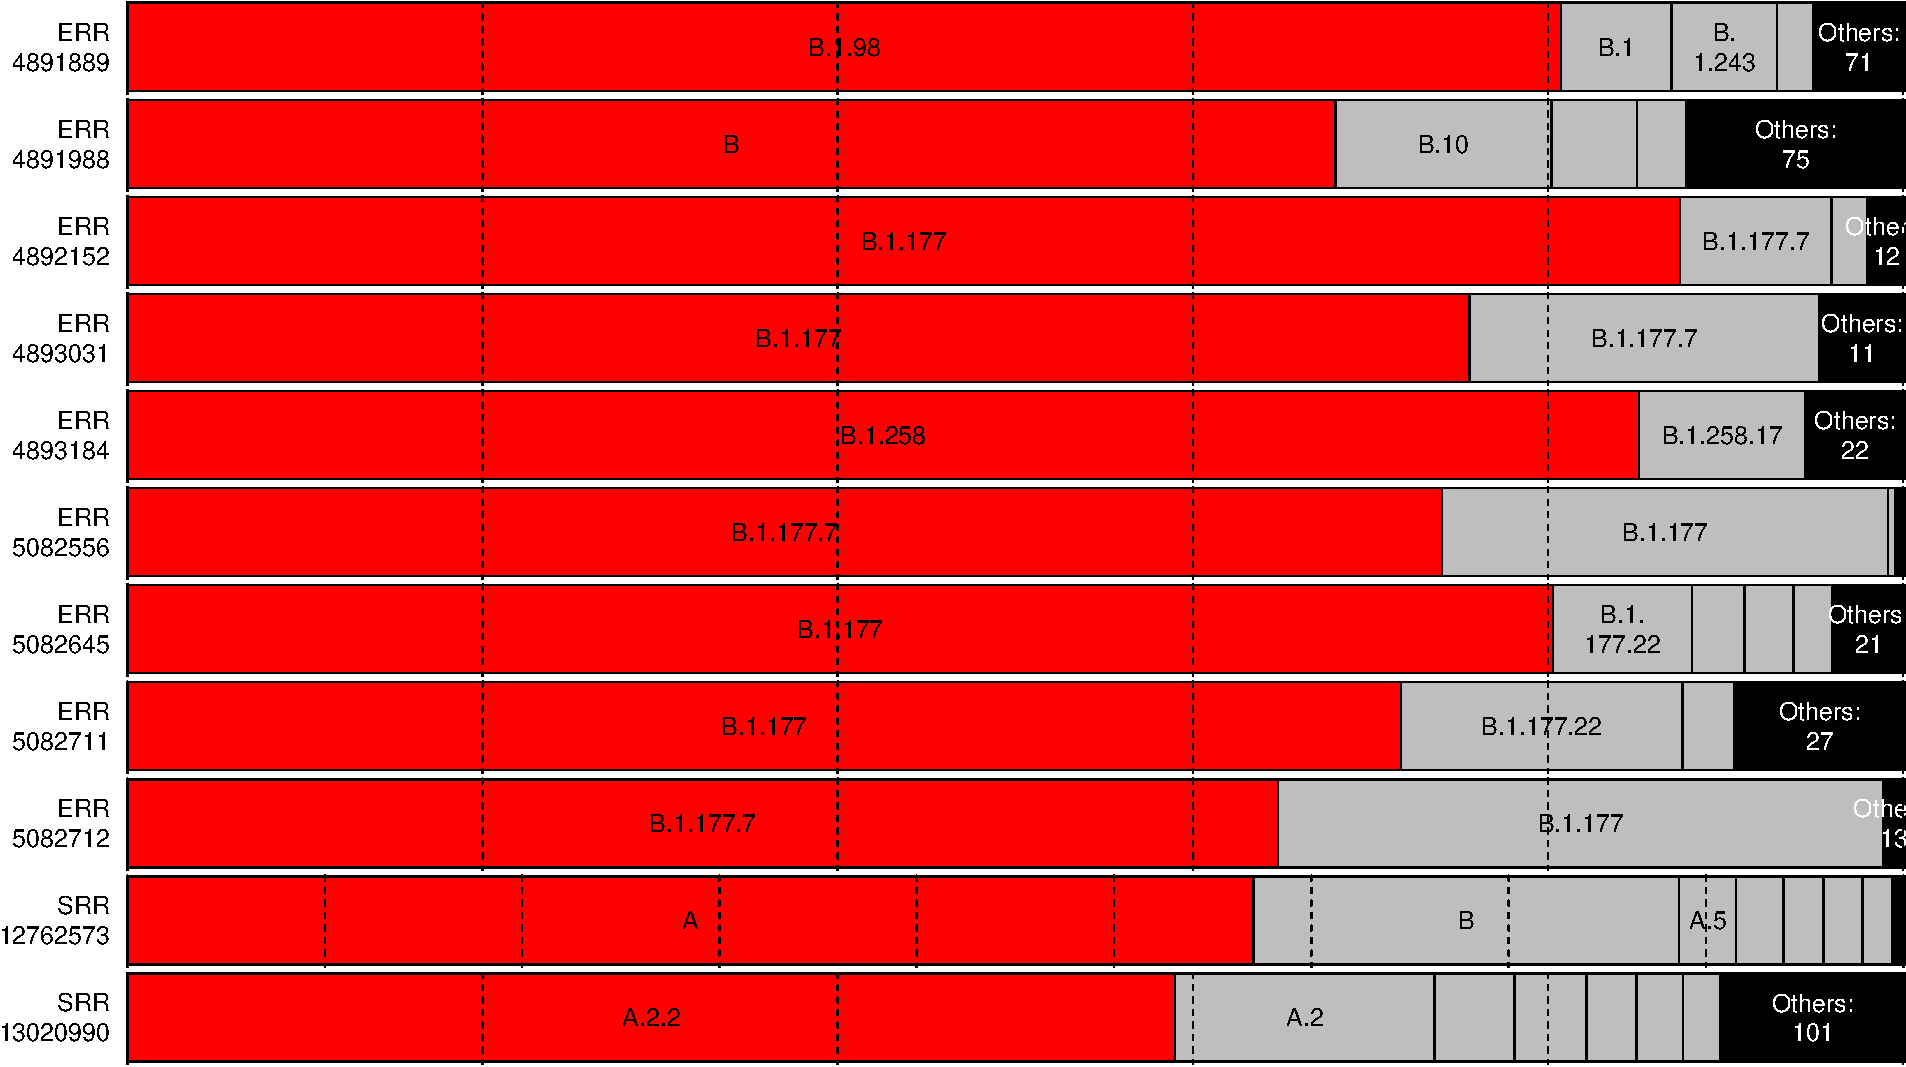
\includegraphics{pangolin_results_report_d_files/figure-latex/pareto-1.pdf}

\hypertarget{probability-bars}{%
\section{Probability Bars}\label{probability-bars}}

\begin{Shaded}
\begin{Highlighting}[]
\NormalTok{boots \textless{}{-}}\StringTok{ }\KeywordTok{vector}\NormalTok{(}\DataTypeTok{mode =} \StringTok{"list"}\NormalTok{, }\DataTypeTok{length =} \KeywordTok{length}\NormalTok{(taxons))}
\KeywordTok{par}\NormalTok{(}\DataTypeTok{mfrow =} \KeywordTok{c}\NormalTok{(}\DecValTok{6}\NormalTok{,}\DecValTok{6}\NormalTok{))}
\ControlFlowTok{for}\NormalTok{(i }\ControlFlowTok{in} \DecValTok{1}\OperatorTok{:}\KeywordTok{length}\NormalTok{(taxons))\{}
    \CommentTok{\# Find modal lineage}
\NormalTok{    thistab \textless{}{-}}\StringTok{ }\KeywordTok{table}\NormalTok{(lins}\OperatorTok{$}\NormalTok{lineage[lins}\OperatorTok{$}\NormalTok{taxon }\OperatorTok{==}\StringTok{ }\NormalTok{taxons[i]])}
\NormalTok{    maxtab \textless{}{-}}\StringTok{ }\KeywordTok{names}\NormalTok{(thistab)[}\KeywordTok{which.max}\NormalTok{(thistab)]}
    \CommentTok{\# Record "probability" for all sequences labelled with this lineage}
\NormalTok{    boots[[i]] \textless{}{-}}\StringTok{ }\NormalTok{lins}\OperatorTok{$}\NormalTok{probability[lins}\OperatorTok{$}\NormalTok{taxon }\OperatorTok{==}\StringTok{ }\NormalTok{taxons[i] }\OperatorTok{\&}\StringTok{ }
\StringTok{            }\NormalTok{lins}\OperatorTok{$}\NormalTok{lineage }\OperatorTok{==}\StringTok{ }\NormalTok{maxtab]}
    
    \CommentTok{\# histogram of probabilities of that lineage}
    \KeywordTok{hist}\NormalTok{(boots[[i]], }\DataTypeTok{breaks =} \KeywordTok{seq}\NormalTok{(}\DecValTok{0}\NormalTok{, }\DecValTok{1}\NormalTok{, }\FloatTok{0.05}\NormalTok{), }
        \DataTypeTok{xlim =} \KeywordTok{c}\NormalTok{(}\DecValTok{0}\NormalTok{, }\DecValTok{1}\NormalTok{))}
    \CommentTok{\# Add a line for the number of genomes that actually had that lineage}
    \KeywordTok{abline}\NormalTok{(}\DataTypeTok{v =} \KeywordTok{mean}\NormalTok{(lins}\OperatorTok{$}\NormalTok{lineage[lins}\OperatorTok{$}\NormalTok{taxon }\OperatorTok{==}\StringTok{ }\NormalTok{taxons[i]] }\OperatorTok{==}\StringTok{ }\NormalTok{maxtab),}
        \DataTypeTok{col =} \DecValTok{2}\NormalTok{, }\DataTypeTok{lwd =} \DecValTok{3}\NormalTok{)}
\NormalTok{\}}
\end{Highlighting}
\end{Shaded}

\includegraphics{pangolin_results_report_d_files/figure-latex/probbars-1.pdf}

\hypertarget{scatterplot}{%
\section{Scatterplot}\label{scatterplot}}

\begin{Shaded}
\begin{Highlighting}[]
\NormalTok{gglist \textless{}{-}}\StringTok{ }\KeywordTok{list}\NormalTok{()}
\ControlFlowTok{for}\NormalTok{(i }\ControlFlowTok{in} \DecValTok{1}\OperatorTok{:}\KeywordTok{length}\NormalTok{(taxons))\{}
\NormalTok{    pang \textless{}{-}}\StringTok{ }\NormalTok{lins[lins}\OperatorTok{$}\NormalTok{taxon }\OperatorTok{==}\StringTok{ }\NormalTok{taxons[i], ]}
\NormalTok{    pang2 \textless{}{-}}\StringTok{ }\KeywordTok{lapply}\NormalTok{(}\KeywordTok{unique}\NormalTok{(pang}\OperatorTok{$}\NormalTok{lineage), }\ControlFlowTok{function}\NormalTok{(x) \{}
        \KeywordTok{data.frame}\NormalTok{(}\DataTypeTok{lineage =}\NormalTok{ x, }
            \DataTypeTok{prop =} \KeywordTok{mean}\NormalTok{(pang}\OperatorTok{$}\NormalTok{lineage }\OperatorTok{==}\StringTok{ }\NormalTok{x))}
\NormalTok{    \}) }\OperatorTok{\%\textgreater{}\%}\StringTok{ }
\StringTok{        }\KeywordTok{bind\_rows}\NormalTok{() }\OperatorTok{\%\textgreater{}\%}\StringTok{ }
\StringTok{        }\KeywordTok{right\_join}\NormalTok{(pang, }\DataTypeTok{by =} \StringTok{"lineage"}\NormalTok{)}
    \CommentTok{\#pang2}
    \KeywordTok{ggplot}\NormalTok{(pang2) }\OperatorTok{+}\StringTok{ }
\StringTok{        }\KeywordTok{aes}\NormalTok{(}\DataTypeTok{x =}\NormalTok{ prop, }\DataTypeTok{y =}\NormalTok{ probability,}
            \DataTypeTok{colour =}\NormalTok{ lineage, }\DataTypeTok{label =}\NormalTok{ lineage) }\OperatorTok{+}\StringTok{ }
\StringTok{        }\KeywordTok{geom\_point}\NormalTok{() }\OperatorTok{+}
\StringTok{        }\CommentTok{\#geom\_text\_repel() + }
\StringTok{        }\KeywordTok{theme}\NormalTok{(}\DataTypeTok{legend.position =} \StringTok{"none"}\NormalTok{)}
    
\NormalTok{    pangtab \textless{}{-}}\StringTok{ }\NormalTok{pang2 }\OperatorTok{\%\textgreater{}\%}\StringTok{ }
\StringTok{        }\KeywordTok{group\_by}\NormalTok{(prop, lineage) }\OperatorTok{\%\textgreater{}\%}\StringTok{ }
\StringTok{        }\KeywordTok{summarise}\NormalTok{(}\DataTypeTok{y =} \DecValTok{1}\NormalTok{, }\DataTypeTok{count =} \KeywordTok{n}\NormalTok{(), }\DataTypeTok{.groups =} \StringTok{"drop"}\NormalTok{) }\OperatorTok{\%\textgreater{}\%}\StringTok{ }
\StringTok{        }\KeywordTok{filter}\NormalTok{(prop }\OperatorTok{\textgreater{}}\StringTok{ }\FloatTok{0.025}\NormalTok{)}
    
\NormalTok{    gglist[[i]] \textless{}{-}}\StringTok{ }\NormalTok{pang2 }\OperatorTok{\%\textgreater{}\%}\StringTok{ }
\StringTok{        }\CommentTok{\# round to nearest 0.5}
\StringTok{        }\CommentTok{\#mutate(prop = round(prop*2, 1)/2,}
\StringTok{        }\CommentTok{\#    probability = round(probability*2, 1)/2) \%\textgreater{}\% }
\StringTok{        }\KeywordTok{group\_by}\NormalTok{(prop, probability, lineage) }\OperatorTok{\%\textgreater{}\%}\StringTok{ }
\StringTok{        }\KeywordTok{summarise}\NormalTok{(}\DataTypeTok{count =} \KeywordTok{n}\NormalTok{(), }\DataTypeTok{.groups =} \StringTok{"drop"}\NormalTok{) }\OperatorTok{\%\textgreater{}\%}\StringTok{ }
\StringTok{        }\KeywordTok{ggplot}\NormalTok{() }\OperatorTok{+}\StringTok{ }\KeywordTok{theme\_bw}\NormalTok{() }\OperatorTok{+}\StringTok{ }
\StringTok{        }\KeywordTok{aes}\NormalTok{(}\DataTypeTok{x =}\NormalTok{ prop, }\DataTypeTok{y =}\NormalTok{ probability, }\DataTypeTok{colour =}\NormalTok{ lineage, }
            \DataTypeTok{label =}\NormalTok{ count) }\OperatorTok{+}\StringTok{ }
\StringTok{        }\KeywordTok{geom\_text}\NormalTok{() }\OperatorTok{+}\StringTok{ }
\StringTok{        }\KeywordTok{theme}\NormalTok{(}\DataTypeTok{legend.position =} \StringTok{"none"}\NormalTok{) }\OperatorTok{+}
\StringTok{        }\KeywordTok{annotate}\NormalTok{(}\StringTok{"text"}\NormalTok{, }\DataTypeTok{x =}\NormalTok{ pangtab}\OperatorTok{$}\NormalTok{prop, }\DataTypeTok{y =} \DecValTok{1}\NormalTok{, }
            \DataTypeTok{label =}\NormalTok{ pangtab}\OperatorTok{$}\NormalTok{lineage,}
            \DataTypeTok{hjust =} \FloatTok{0.5}\NormalTok{, }\DataTypeTok{vjust =} \DecValTok{{-}1}\NormalTok{) }\OperatorTok{+}
\StringTok{        }\KeywordTok{labs}\NormalTok{(}\DataTypeTok{x =} \StringTok{"Proportion of Lineage"}\NormalTok{,}
            \DataTypeTok{y =} \StringTok{"Bootstrap Probability"}\NormalTok{,}
            \DataTypeTok{title =} \OtherTok{NULL}\NormalTok{) }\OperatorTok{+}
\StringTok{        }\KeywordTok{scale\_x\_continuous}\NormalTok{(}\DataTypeTok{breaks =} \KeywordTok{seq}\NormalTok{(}\DecValTok{0}\NormalTok{,}\DecValTok{1}\NormalTok{,}\FloatTok{0.1}\NormalTok{)) }\OperatorTok{+}
\StringTok{        }\KeywordTok{scale\_y\_continuous}\NormalTok{(}\DataTypeTok{breaks =} \KeywordTok{seq}\NormalTok{(}\DecValTok{0}\NormalTok{,}\FloatTok{1.1}\NormalTok{,}\FloatTok{0.1}\NormalTok{)) }\OperatorTok{+}
\StringTok{        }\KeywordTok{coord\_cartesian}\NormalTok{(}\DataTypeTok{ylim =} \KeywordTok{c}\NormalTok{(}\DecValTok{0}\NormalTok{, }\FloatTok{1.1}\NormalTok{)) }\OperatorTok{+}\StringTok{ }
\StringTok{        }\KeywordTok{geom\_abline}\NormalTok{(}\DataTypeTok{slope =} \DecValTok{1}\NormalTok{, }\DataTypeTok{intercept =} \DecValTok{0}\NormalTok{)}
\NormalTok{\}}
\NormalTok{cowplot}\OperatorTok{::}\KeywordTok{plot\_grid}\NormalTok{(}\DataTypeTok{plotlist =}\NormalTok{ gglist)}
\end{Highlighting}
\end{Shaded}

\includegraphics{pangolin_results_report_d_files/figure-latex/ggscatter-1.pdf}

\end{document}
